\documentclass[12pt]{article}

\usepackage{amsmath}
\usepackage[margin = 1in]{geometry}
\usepackage{graphicx}
\usepackage{booktabs}
\usepackage{natbib}
\usepackage{indentfirst}
\usepackage{float}
\usepackage{lineno}
\setlength{\emergencystretch}{3em}

\linenumbers

\usepackage{setspace}
\doublespacing
\usepackage[colorlinks=true, citecolor=blue]{hyperref}

\usepackage{color}
\newcommand{\blue}{\color{blue}}

\title{Forecasting Protest Escalation into Political Violence in Latin America}
\author{Sonia Lucey}
\sloppy
\begin{document}
\maketitle


\begin{abstract}
This paper develops and evaluates a forecasting framework designed to predict whether protest activity in Latin America escalates into political violence at the country--month level. Using ACLED event data from 2015--2025, a protest-conditional dataset is constructed that models escalation from month $t$ to month $t+1$. Structural economic and political variables are merged from the World Bank and the Democracy Index. Logistic regression and gradient boosted tree models are estimated and evaluated using temporal out-of-sample validation. Results indicate that escalation is strongly path dependent; recent violence levels and protest momentum are more influential than structural macroeconomic variables on a monthly basis. Nonlinear modeling improves predictive performance relative to logistic regression, although overall forecasting accuracy remains moderate. The findings highlight both the strengths and limitations of short-term political violence forecasting in high protest environments. The framework reframes conflict forecasting as a transition problem rather than an incidence problem.

\noindent\textbf{Keywords}: early warning systems, event data, path dependence, probabilistic forecasting, temporal dynamics

\end{abstract}

\section{Introduction}
\label{sec:intro}

Forecasting political violence remains one of the most challenging problems in applied political data science \citep{mueller2024conflict,hegre2019views}. Intelligence and policy organizations seek to anticipate political violence before it escalates, rather than simply explaining it after the fact. Traditional approaches to early warning have often focused on identifying countries at risk of instability using structural indicators. Although these approaches have provided valuable information, they often treat political violence as a standalone outcome and overlook the dynamic processes through which violence emerges \citep{hegre2019views}.

In reality, political violence rarely occurs without warning. Episodes of violence are often preceded by periods of social unrest, including protests, strikes, and demonstrations \citep{acled2019}. These environments create conditions in which violence can escalate or remain peaceful depending on political, economic, and institutional responses. Although advances in event data and machine learning have improved predictive performance, the onset and escalation of violence remain difficult to anticipate with high accuracy \citep{mueller2024conflict}. Although political violence remains relatively infrequent, Latin America is characterized by high levels of protest activity, making it increasingly important to understand when protests escalate into violence. Most forecasting models predict conflict incidence without conditioning on protest activity. The relevant question is therefore not whether protest occurs, but whether protest escalates into violence. This paper focuses on forecasting the escalation of protest into political violence at the country–month level.

Conditional on protest activity in month $t$, the central research question is: 
\textit{What is the probability that violence occurs or increases substantially in month $t+1$?} By restricting the sample to protest months, the framework isolates escalation dynamics, shifting the problem from predicting baseline violence risk to modeling short-run deterioration.

The importance of this research lies in its direct relevance for operational early warning. Policymakers and institutions that monitor protests require tools that distinguish routine civic demonstrations from protests with elevated escalation risk. By modeling transition risk rather than the prevalence of structural conflict, this framework aligns more directly with the practical needs of monitoring systems \citep{hegre2019views}.

Existing literature has shown that event data such as ACLED can be useful for conflict forecasting, and that structural indicators can help identify broader instability risk \citep{acled2019,mueller2024conflict}. However, much of this literature focuses on violence incidence in general rather than protest-conditional escalation. In regions such as Latin America, where protest is common, a model that does not condition on protest may conflate the emergence of protest with its deterioration. This leaves a gap between general conflict forecasting and the more specific question of whether an already mobilized environment will worsen.

This paper presents a protest-conditional forecasting framework built on three core principles: protest-conditional sampling, a one-month forecasting horizon, and an emphasis on within-country variation. Together, these principles produce a forecasting framework intended to improve short-run escalation assessment in operational early-warning contexts. To guide the empirical analysis, this study evaluates the following hypotheses:

\textbf{H1}: Higher levels of recent violence are associated with a higher probability that protest activity escalates into political violence in the following month.

\textbf{H2}: Positive changes in protest activity (protest growth) are associated with a higher probability of escalation.

\textbf{H3}: Macroeconomic and institutional variables have weaker effects on escalation at the one-month horizon than short-run conflict dynamics.

The rest of the paper is organized as follows. Section~\ref{sec:data} describes the data and target variable, Section~\ref{sec:meth} outlines the forecasting methodology, Section~\ref{sec:resu} presents the results, and Section~\ref{sec:disc} discusses interpretation, limitations, and policy implications.

\section{Data Description}
\label{sec:data}

This section describes the data used to answer the research question of whether protest activity in Latin America escalates into political violence in the following month.

\subsection{Event Data}

Data on political violence and protest events from Armed Conflict Location \& Event Data (ACLED) serve as the basis for escalation forecasting, consistent with previous work showing their utility in conflict models \citep{rod2024protest_forecasting}. ACLED provides geocoded records of protest and violent events. Events are aggregated to the country--month level for Latin American countries between 2015 and 2025. Violence includes organized armed confrontations and one-sided violence against civilians. Monthly aggregation balances temporal resolution and statistical stability.

Descriptive statistics for key variables are reported in Table~\ref{tab:summary_stats}.

\begin{table}[h!]
\centering
\caption{Summary statistics for key variables}
\label{tab:summary_stats}
\begin{tabular}{lcccc}
\toprule
Variable & Mean & Std. Dev. & Min & Max \\
\midrule
Protest Count & 82.77 & 140.22 & 1 & 3417 \\
Violence Count & 53.85 & 99.09 & 0 & 601 \\
Protest Growth & -0.31 & 153.01 & -3267 & 2856 \\
\bottomrule
\end{tabular}
\end{table}

Protest and violence counts exhibit wide variation, with large differences between typical and extreme values, indicating periods of high-intensity events. Protest growth shows considerable variability, with both large positive and negative changes, reflecting sharp fluctuations in protest activity over time.


\subsection{Protest-Conditional Sampling}

The sample is restricted to country–months with at least one protest event to isolate escalation dynamics rather than model protest emergence. Including all country–months would conflate two distinct processes—protest occurrence and escalation into violence—which are driven by different mechanisms \citep{mueller2024conflict}. Protest emergence often reflects structural factors such as electoral cycles or economic conditions, whereas escalation captures short-run breakdowns in protest–state interactions and the intensification of collective action.

Conditioning on protest treats mobilization as the baseline political environment and focuses the model on transitions from protest to violence. This aligns with early-warning objectives, which prioritize identifying which protest episodes are most likely to escalate rather than predicting protest itself \citep{hegre2019views}. It also clarifies the outcome by excluding violence unrelated to protest and improves comparability across countries by removing structural zeros from non-protest months. As a result, the forecasting task shifts from predicting violence incidence to distinguishing higher- and lower-risk protest environments.

\subsection{Target Variable}

The dependent variable measures whether protest activity escalates into political violence in the following month. Escalation is defined as a meaningful deterioration in conflict dynamics, capturing both the onset of violence and the intensification of existing violence. This definition is designed to capture both extensive and intensive margins of conflict dynamics.

Formally, $\text{Escalation} = 1$ if either:
\begin{enumerate}
\item violence occurs in month $t+1$ when none occurred in month $t$, or
\item $Violence{t+1} \geq 1.5 \times Violence_t$
\end{enumerate}
and $0$ otherwise.

The inclusion of both an onset condition and a proportional increase condition captures two distinct escalation pathways. The first identifies transitions from nonviolent protest environments into violent confrontation, representing a qualitative shift in political interaction. The second captures intensification within already unstable contexts, recognizing that escalation may occur through the rapid amplification of existing violence rather than a shift from zero to positive levels.

A central design decision concerns the 1.5 proportional threshold. Monthly conflict event data contain natural volatility due to reporting delays, clustering of minor incidents, and small fluctuations. Defining escalation as any positive increase would therefore capture routine variation rather than meaningful deterioration, inflating the positive class and weakening the conceptual distinction between stability and escalation. Conversely, a stricter rule, such as doubling violence, would risk overlooking substantively important transitions, particularly in lower-violence contexts where moderate increases may still reflect worsening protest–state relations. This is shown in Table~\ref{tab:threshold_sensitivity}.

\begin{table}[H]
\centering
\caption{Sensitivity of escalation threshold choice}
\label{tab:threshold_sensitivity}
\begin{tabular}{lccc}
\toprule
Threshold & Escalation Rate & Test AUC & Interpretation \\
\midrule
1.25 & 0.343 & 0.739 & Captures noise / minor variation \\
1.50 & 0.269 & 0.778 & Balanced signal vs noise \\
2.00 & 0.204 & 0.837 & Too restrictive, sparse positives \\
\bottomrule
\end{tabular}
\end{table}

The 1.5 multiplier provides an intermediate standard requiring a 50\% increase in violent events relative to the previous month. This rule produces an escalation rate of approximately 27\% among protest months, preserving sufficient variation while maintaining substantive interpretability. It also improves cross-country comparability. Violence levels vary widely across Latin American countries, and absolute thresholds would disproportionately classify higher-violence countries as escalatory. A proportional rule instead evaluates escalation relative to each country’s recent baseline.

Exploratory sensitivity analysis further informed this choice. Lower thresholds yielded escalation rates nearly on par with those in non-escalation months, capturing ordinary volatility rather than meaningful deterioration; higher thresholds produced sparse positive cases and greater estimation instability. The 1.5 multiplier, therefore, provides a practical balance between sensitivity and noise reduction.

Table~\ref{tab:threshold_sensitivity} shows that lower thresholds inflate the positive class by capturing routine fluctuations, while higher thresholds reduce sample size and predictive stability. The 1.5 threshold provides the best balance.

\subsection{Structural Covariates}

Annual macroeconomic and political indicators are merged into the country--month panel to capture structural conditions that may influence escalation risk. The variables included are GDP growth, inflation, unemployment, the Gini coefficient (a measure of income inequality, where higher values indicate greater inequality), and the Democracy Index score.

These variables represent slow-moving economic and institutional characteristics that may shape the broader environment in which protest and violence unfold. While the model's primary focus is short-run transition dynamics, escalation processes may still be conditioned by underlying macroeconomic stress and political institutions.

All structural covariates are available at an annual frequency, while the unit of analysis in this study is the country–month. To align these, annual values are forward-filled across months within each calendar year, meaning that the same annual value is assigned to each month of that year. For example, a country’s 2020 GDP growth rate is used for all months from January through December 2020.

This procedure assumes that structural macroeconomic and institutional conditions change slowly and remain relatively stable within a given year. Given the low-frequency nature of these indicators, this assumption is substantively reasonable for modeling short-run transitions such as month-to-month escalation dynamics.

These data characteristics directly inform the modeling approach. Because violence is not random but tends to persist and cluster over time, lagged measures of violence are included to capture path dependence in conflict dynamics. Similarly, variation in protest intensity over time supports the use of protest growth as a predictor of escalation. Because escalation may involve nonlinear thresholds and interactions, both a linear model (logistic regression) and a nonlinear model (XGBoost) are implemented to assess whether additional predictive structure can be captured beyond simple temporal dynamics.


\section{Methods}
\label{sec:meth}

This section presents the methodologies used to generate the results from the data analysis. Model performance is evaluated using ROC AUC and PR AUC, which capture discrimination in the presence of class imbalance (see Section~\ref{sec:forecast_perf}). Because the objective is out-of-sample prediction rather than causal inference, model design emphasizes temporal integrity, avoidance of information leakage, and robustness to serial and spatial dependence. All predictors used in the final models include lagged violence measures, protest dynamics, and recent violence indicators.

Lagged violence measures include 
\emph{violence\_count\_lag1}, \emph{violence\_count\_lag2}, and 
\emph{violence\_rolling3}. Protest dynamics are captured by 
\emph{protest\_growth}, and recent violence indicators by 
\emph{recent\_violence}. Protest growth is defined as the change in protest counts from month \(t-1\) to month \(t\). The recent violence indicator equals 1 if any violent event occurred in month \(t\), and 0 otherwise. All continuous predictors are demeaned by country using training-period means, producing variables denoted with a “\emph{\_dm}” suffix.

\subsection{Data Processing and Feature Engineering}

Countries in Latin America differ substantially in their baseline levels of violence, institutional stability, and protest frequency. A forecasting model trained on pooled country--month observations may learn that certain countries are persistently high-risk while others are persistently low-risk. Such cross-sectional differences can artificially inflate predictive performance without capturing meaningful escalation dynamics.

For each country $i$, time period $t$, and predictor $X_{it}$, define $\bar{X}_{i,\text{train}}$ as the country-specific mean of $X_{it}$ computed over the training sample. The demeaned predictor is given by
\[
\tilde{X}_{it} = X_{it} - \bar{X}_{i,\text{train}}.
\]

This procedure isolates within-country temporal variation and ensures that the model learns deviations from a country’s historical baseline rather than persistent structural differences. Importantly, training-set means are applied to the validation and test sets without recalculating, preventing information from future periods from entering the model estimation.

All lagged variables are constructed using only information available at time $t$, ensuring no forward-looking bias. These feature construction steps form the basis for all subsequent model estimation and interpretation, including forecast performance (Section~\ref{sec:forecast_perf}), feature importance (Section~\ref{sec:feature_imp}), and substantive patterns (Section~\ref{sub_pat}).

\begin{table}[H]
\centering
\caption{Key model features}
\begin{tabular}{ll}
\toprule
Variable & Description \\
\midrule
violence\_count\_lag1 & Violence in month $t$ \\
violence\_count\_lag2 & Violence in month $t-1$ \\
violence\_rolling3 & 3-month average violence \\
protest\_growth & Change in protest count from $t-1$ to $t$ \\
recent\_violence & Indicator for recent violence presence \\
democracy\_index & Annual democracy score (forward-filled) \\
inflation\_lag1 & Lagged inflation rate \\
\bottomrule
\end{tabular}
\end{table}

\subsection{Model Specification}

The baseline model employs logistic regression to estimate the probability of escalation:
$$
P(Escalation_t = 1 \mid X_t) = \frac{1}{1 + e^{-X_t\beta}}.
$$

Logistic regression is appropriate given the binary nature of the dependent variable. It provides interpretable marginal effects and probabilistic outputs, which are essential in early-warning contexts where decision-makers require calibrated risk estimates rather than binary classifications.

Escalation processes exhibit strong path dependence. Violence often follows violence through retaliation cycles, repression spirals, or strategic signaling among actors. To capture these dynamics, lagged violence counts and measures of protest growth are included. Lagged violence measures represent recent instability and capture the conflict-trap dynamic, whereby past violence increases the likelihood of future violence. Protest growth captures momentum effects in mobilization.

To complement the linear logistic model, a nonlinear specification using Extreme Gradient Boosting (XGBoost) is implemented. Gradient boosted trees construct an ensemble of sequential decision trees that iteratively minimize classification error. XGBoost handles nonlinearities and interactions automatically and incorporates regularization to mitigate overfitting. Both models are evaluated to assess whether nonlinear structure materially improves predictive performance, as reflected in forecast performance results (Section~\ref{sec:forecast_perf}) and feature importance (Section~\ref{sec:feature_imp}).

\subsection{Training and Validation Design}

A central concern in forecasting political violence is preserving temporal integrity. Random cross-validation would mix future observations into training folds, introducing look-ahead bias.

Instead, the dataset is split chronologically to preserve temporal integrity and avoid look-ahead bias. The training set includes observations from 2015--2022, the validation set consists of 2023 data used for hyperparameter tuning, and the test set contains the most recent period (2024--2025). Hyperparameters for XGBoost are selected based on validation-set performance measured by area under the ROC curve (AUC), and the final model is evaluated on the held-out test set (Section~\ref{sec:forecast_perf}).

\subsection{Forecast Evaluation Metrics}

Model performance is evaluated using ROC AUC and precision--recall AUC. The AUC measures the model’s ability to discriminate between escalation and non-escalation months across all possible probability thresholds. Precision--recall AUC is used because escalation events are relatively infrequent, making it more informative in imbalanced settings. These metrics are reported in Section~\ref{sec:forecast_perf}, while threshold-based performance is further examined using precision--recall curves (Section~\ref{sec:pr}).

\subsection{Risk Distribution and Spatial Visualization}

While the model is estimated at the country--month level, predicted escalation probabilities are mapped to geographic grid cells using the underlying ACLED event coordinates. This allows model outputs to be interpreted spatially, highlighting geographic clustering of escalation risk. The resulting spatial risk distribution is presented in Section~\ref{sec:risk_dist}. Because the statistical models are estimated at the country--month level, this mapping is descriptive rather than a separate sub-national model.

\subsection{Model Diagnostics (Precision--Recall and Calibration)}

Model diagnostics include precision--recall curves and calibration plots. Precision--recall curves evaluate model performance across probability thresholds, particularly in imbalanced settings (Section~\ref{sec:pr}). Calibration plots compare predicted escalation probabilities with observed escalation rates across probability bins to assess how well predicted probabilities correspond to realized outcomes (Section~\ref{sec:model_cali}).

\subsection{Feature Importance}

To interpret the nonlinear model, feature importance scores from the XGBoost model are used. These scores identify which predictors contribute most strongly to escalation prediction, as reported in Section~\ref{sec:feature_imp}.

\subsection{Substantive Interpretation}

Because the model includes several correlated measures of recent violence, individual coefficients are interpreted as conditional partial associations rather than standalone effects. The analysis focuses on overall patterns of predictive importance rather than isolated coefficient magnitudes, with substantive implications discussed in Section~\ref{sub_pat}.


\section{Results}
\label{sec:resu}

This section reports the results generated from the methods discussed in Section~\ref{sec:meth}. Model performance is evaluated using out-of-sample metrics on chronologically separated validation and test sets.

\subsection{Forecast Performance}
\label{sec:forecast_perf}

Because the objective is probabilistic forecasting of a binary outcome, the primary evaluation metric is the area under the receiver operating characteristic curve (AUC-ROC). The AUC measures the model’s ability to discriminate between escalation and non-escalation months across all possible probability thresholds. An AUC of 0.50 corresponds to random guessing. At the same time, an AUC of 1.00 reflects perfect discrimination, meaning that the model assigns a higher predicted probability to every escalation month than to every non-escalation month.

Table \ref{tab:model_comp} summarizes out-of-sample forecasting performance across model specifications.

\begin{table}[H]
\centering
\caption{Model comparison}
\label{tab:model_comp}
\begin{tabular}{lccc}
\toprule
Model & Validation AUC & Test AUC & PR AUC \\
\midrule
Baseline (Recent Violence) & -- & 0.578 & -- \\
Logistic Regression & 0.531 & 0.585 & 0.351 \\
XGBoost (tuned) & 0.61 & 0.673 & 0.39 \\
\bottomrule
\end{tabular}
\end{table}

These results indicate that while nonlinear modeling captures additional structure, most of the predictive signal is already captured by simple lag-based dynamics. The baseline model using only recent violence achieves a test AUC of 0.578. The full logistic regression model provides only a modest improvement, with validation AUC 0.531 and test AUC 0.585. The precision–recall AUC on the test set is 0.351, indicating moderate predictive performance in an imbalanced setting. Because escalation events are relatively infrequent, the model faces a tradeoff between correctly identifying true escalation cases (recall) and avoiding false positives (precision). Differences between validation and test performance reflect normal temporal variation rather than evidence of overfitting. Importantly, all specifications exceed random classification (AUC = 0.50), indicating that they capture a meaningful signal in escalation risk.  

XGBoost provides a clear improvement over logistic regression (Test AUC 0.673 vs. 0.585), although overall predictive performance remains moderate. Given the inherent stochasticity of political violence, even modest improvements over random classification are substantively meaningful.

The concentration of predictive power in lagged variables, as reflected in the modest performance gains over the baseline model (Table~\ref{tab:model_comp}) and the dominance of lagged violence measures in the XGBoost feature importance rankings (Figure~\ref{fig:xgbimportance}), indicates that escalation is primarily driven by recent instability, with limited predictive signal available before its emergence. This suggests inherent constraints on early-warning forecasting. Consistent with this, the modest performance gains relative to the baseline model indicate that short-run dynamics—particularly recent violence—account for most of the model’s predictive power.

\begin{table}[H]
\centering
\caption{Logistic regression inference results for short-term escalation}
\label{tab:logit_inference}
\begin{tabular}{lcccc}
\toprule
Variable & Coefficient & Std. Error & 95\% CI & p-value \\
\midrule
Violence count, lag 1 & -0.011 & 0.006 & [-0.022,\ 0.001] & 0.070 \\
Protest count & -0.006 & 0.001 & [-0.009,\ -0.003] & $<0.001$ \\
Democracy Index & 0.221 & 0.078 & [0.067,\ 0.374] & 0.005 \\
Region violence mean & 0.003 & 0.004 & [-0.004,\ 0.011] & 0.379 \\
\bottomrule
\end{tabular}
\end{table}

Lagged violence is marginally significant (p = 0.070), and its 95\% confidence interval [-0.022, 0.001] narrowly includes zero, indicating uncertainty about the direction and strength of its effect at conventional significance levels.

These findings do not imply that protest episodes are short-lived; rather, they indicate that at a one-month forecasting horizon, the information relevant for predicting escalation is concentrated in the most recent period. Ongoing protest dynamics are already captured by contemporaneous measures such as protest counts and recent violence, limiting the additional contribution of longer lags.

The protest count is statistically significant $(p < 0.001)$, with a confidence interval of $[-0.009, -0.003]$ that lies entirely below zero, indicating that higher protest activity is associated with a lower probability of escalation, holding other factors constant. Similarly, the Democracy Index is statistically significant $(p = 0.005)$, and its confidence interval $[0.067, 0.374]$ lies entirely above zero, indicating that more democratic countries are associated with a higher probability of escalation, conditional on protests.

The regional violence mean is not statistically significant $(p = 0.379)$, and its confidence interval $[-0.004, 0.011]$ includes zero, suggesting no clear independent effect once recent conflict dynamics and institutional conditions are accounted for. Because several predictors capture closely related aspects of instability, coefficients should be interpreted as conditional associations rather than standalone effects. Overall, the results reinforce the central role of recent violence in shaping escalation risk, although its predictive influence appears distributed across correlated features rather than concentrated in a single variable.

\subsection{Risk Distribution}
\label{sec:risk_dist}

While the model is estimated at the country–month level, escalation dynamics are inherently spatial and often occur at sub-national scales. To complement the temporal evaluation of model performance, predicted probabilities are mapped onto geographic grid cells using the underlying event locations from ACLED, rather than being independently estimated at the sub-national level. This approach allows the model’s outputs to be interpreted not only in terms of \textit{when} escalation is likely to occur, but also \textit{where} it is most likely to emerge. The resulting visualization translates country-level forecasts into a spatial risk surface, highlighting geographic clustering and localized hotspots of escalation risk.

Figure~\ref{fig:risk_map} illustrates this spatial distribution of predicted escalation risk across sub-national grid cells. Darker areas indicate higher predicted probabilities of protest escalation into violence. Consistent with the overall distribution of outcomes, most country–month observations are associated with relatively low predicted risk, reflecting the fact that escalation occurs in a minority of protest months.

\subsection{Precision--Recall and Risk Ranking}
\label{sec:pr}

While overall discrimination is modest, additional insight can be gained by examining model performance across probability thresholds. Figure~\ref{fig:prcurve} presents the precision--recall curve for the logistic 
regression model on the test dataset. Precision--recall curves are particularly 
useful when the outcome variable is imbalanced, meaning that the positive class (escalation) represents a relatively small share of observations compared to the negative class. Because escalation occurs in 
roughly 27\% of protest months, the precision--recall tradeoff provides insight 
into how well the model identifies escalation events among higher-risk 
predictions.


The model demonstrates improved precision in higher predicted-risk ranges, indicating that months flagged as high risk are more likely than baseline to experience escalation. This suggests that risk ranking rather than binary classification may be the most appropriate operational use of the model.

\subsection{Model Calibration}
\label{sec:model_cali}

Calibration evaluates whether predicted probabilities correspond to observed 
outcomes. Figure~\ref{fig:calibration} compares predicted escalation risk with 
observed escalation rates across probability bins.

A well-calibrated model should produce points that lie close to the 45-degree line, indicating that predicted probabilities align with observed escalation 
frequencies.

Figure~\ref{fig:calibration} shows that the model is imperfectly calibrated, with predicted probabilities not consistently aligning with observed escalation rates. At lower predicted risk levels, the model slightly overpredicts risk, as observed escalation rates fall below predicted values. In the mid-range of predicted probabilities, the relationship becomes more irregular, reflecting noise and limited observations within bins. At higher predicted risk levels, the model tends to underpredict escalation, as observed rates exceed predicted probabilities.

Overall, the model captures the general upward relationship between predicted risk and observed escalation, indicating that higher predicted probabilities correspond to higher realized risk. However, deviations from the 45-degree line suggest that the predicted probabilities should be interpreted as relative risk rankings rather than precise probability estimates.

\subsection{Feature Importance}
\label{sec:feature_imp}
Figure~\ref{fig:xgbimportance} displays the top predictors identified by the
XGBoost model. The feature importance scores indicate which variables
contribute most strongly to escalation prediction. For example, \textit{violence\_rolling3} represents the three-month average of violence counts, while \textit{recent\_violence\_dm} reflects deviations from a country’s baseline violence level.

Figure~\ref{fig:xgbimportance} shows that lagged violence measures dominate the model’s feature importance rankings, indicating that recent conflict dynamics are the most informative predictors of escalation. The most important variable, \textit{violence\_rolling3}, captures sustained recent instability, while \textit{recent\_violence\_dm} and lagged violence counts (\textit{violence\_count\_lag1, lag2}) further reinforce the importance of short-run conflict persistence.

Measures of protest dynamics, including \textit{protest\_growth} and \textit{protest\_acceleration}, also contribute to prediction, though to a lesser extent. These variables capture momentum in mobilization, suggesting that rapid increases in protest activity are associated with elevated escalation risk.

In contrast, structural and macroeconomic variables (e.g., inflation, regional averages) play a more limited role, consistent with the expectation that slow-moving factors are less informative at short forecasting horizons. Overall, these results reinforce the central role of recent conflict dynamics in shaping escalation risk.

\subsection{Substantive Patterns}
\label{sub_pat}

Across specifications, lagged violence is the strongest predictor of escalation, consistent with path dependence and conflict persistence. Conflict exhibits persistence, with past violence increasing the likelihood of future escalation through mechanisms such as retaliation, repression, and strategic signaling among actors. Protest growth also contributes to predictions, as rapid increases in mobilization are associated with a higher risk of escalation, supporting a momentum-driven view in which intensifying protest strains state capacity.

By contrast, structural macroeconomic variables—such as GDP growth, inflation, unemployment, inequality, and democracy scores—have limited predictive power at a one-month horizon. While the nonlinear XGBoost model improves predictive performance relative to logistic regression, overall accuracy remains moderate, suggesting that most predictive signal is captured by short-run dynamics, particularly lagged violence and protest momentum.

Overall, empirical findings align closely with the study’s theoretical expectations, providing strong support for H1, moderate support for H2, and evidence consistent with H3.

\section{Discussion}
\label{sec:disc}

\subsection{Interpretation of Escalation Dynamics}

The results indicate that escalation from protest to violence is strongly path dependent. Recent periods of instability are associated with a higher likelihood of subsequent escalation, consistent with self-reinforcing dynamics such as repression, retaliation, and strategic adaptation by actors. Escalation is therefore not random, but systematically related to recent conflict activity.

Measures of protest intensity further reinforce the importance of short-run dynamics. Increases in protest activity are associated with a higher risk of escalation, suggesting that rapid mobilization may heighten tensions, strain institutional responses, and create conditions in which violence becomes more likely.

In contrast, structural macroeconomic and institutional variables exhibit limited predictive power at the monthly horizon considered in this study. While these factors may shape the broader conditions under which protests emerge, they appear less relevant for explaining short-term transitions from protest to violence. This distinction highlights the importance of temporal scale: escalation dynamics operate over short horizons, whereas structural variables evolve more slowly and may influence longer-run patterns rather than immediate outcomes.

These findings suggest that escalation is best understood as a short-run interaction process driven by recent conflict dynamics rather than by underlying structural conditions. From a practical perspective, this implies that early-warning systems should prioritize real-time indicators of instability, particularly recent violence and changes in protest activity. Although overall predictive performance remains moderate, the model provides meaningful differentiation in risk across observations, making it more useful for identifying relatively high-risk environments than for generating precise probability forecasts. 

\subsection{Robustness and Design Choices}

Several methodological choices ensure that results are not artifacts of modeling decisions. Within-country demeaning removes persistent cross-country differences, the 1.5 escalation threshold balances sensitivity and noise, and the chronological training–validation–test split preserves out-of-sample evaluation. Nonlinear gradient boosting serves as a robustness check, while protest-conditional sampling avoids conflating escalation with protest emergence.

Together, these choices strengthen the credibility of the findings by reducing the risk that results reflect mechanical artifacts rather than substantive patterns.

\subsection{Limitations}

Despite these safeguards, several limitations remain. First, the country--month unit aggregates sub-national dynamics, potentially obscuring localized escalation patterns. Although the ACLED data include event-level latitude and longitude coordinates, and these are used to construct spatial maps of protest and violence, geographic variation within countries is not explicitly incorporated into the regression model. While the spatial maps provide descriptive evidence of clustering and regional patterns, they do not directly inform estimation. As a result, important sub-national heterogeneity in escalation dynamics may be overlooked. Future work could incorporate geospatial features or sub-national units to better capture localized escalation risk. Second, this study relies on publicly available event data, which may be subject to reporting bias. Variation in media coverage and press freedom can affect observed event counts, potentially understating escalation risk in countries with restricted media environments and biasing model predictions downward.

Third, annual macroeconomic indicators--forward-filled to monthly frequency—cannot capture short-term shocks, which may reduce their apparent predictive power. Fourth, the one-month forecasting horizon limits predictive capacity, as escalation is often driven by sudden, unobserved triggers such as policy decisions or police actions. Finally, predictive performance remains modest, reflecting both data constraints and the inherently stochastic and strategic nature of political violence.

\subsection{Policy Implications and Conclusion}

Despite moderate predictive performance, the framework has meaningful implications for early-warning systems. Even modest improvements over random classification can aid prioritization, allowing analysts to focus limited resources on higher-risk protest contexts. The protest-conditional design reflects operational realities in Latin America, where protests are common, and the key question is not whether they occur, but whether they escalate.

The results provide a clear answer to the research question: conditional on protest activity, \textbf{escalation into political violence in the following month is driven primarily by recent violence and protest growth, while structural macroeconomic and institutional conditions play a more limited role at the monthly horizon.}

Future research could extend this framework by incorporating higher-frequency data, subnational modeling, or real-time indicators, such as social media signals, to improve short-term predictive performance.

\section*{Supplemental Materials}

All code and data used in this manuscript are available at \url{https://github.com/snlucey12/forecasting-protest-escalation}. The repository includes data cleaning scripts, model training code, and all figures used in the paper, along with a README file describing how to reproduce the results.

\appendix
\section{Appendix}
\vspace{-0.6cm}

\begin{figure}[H]
\centering
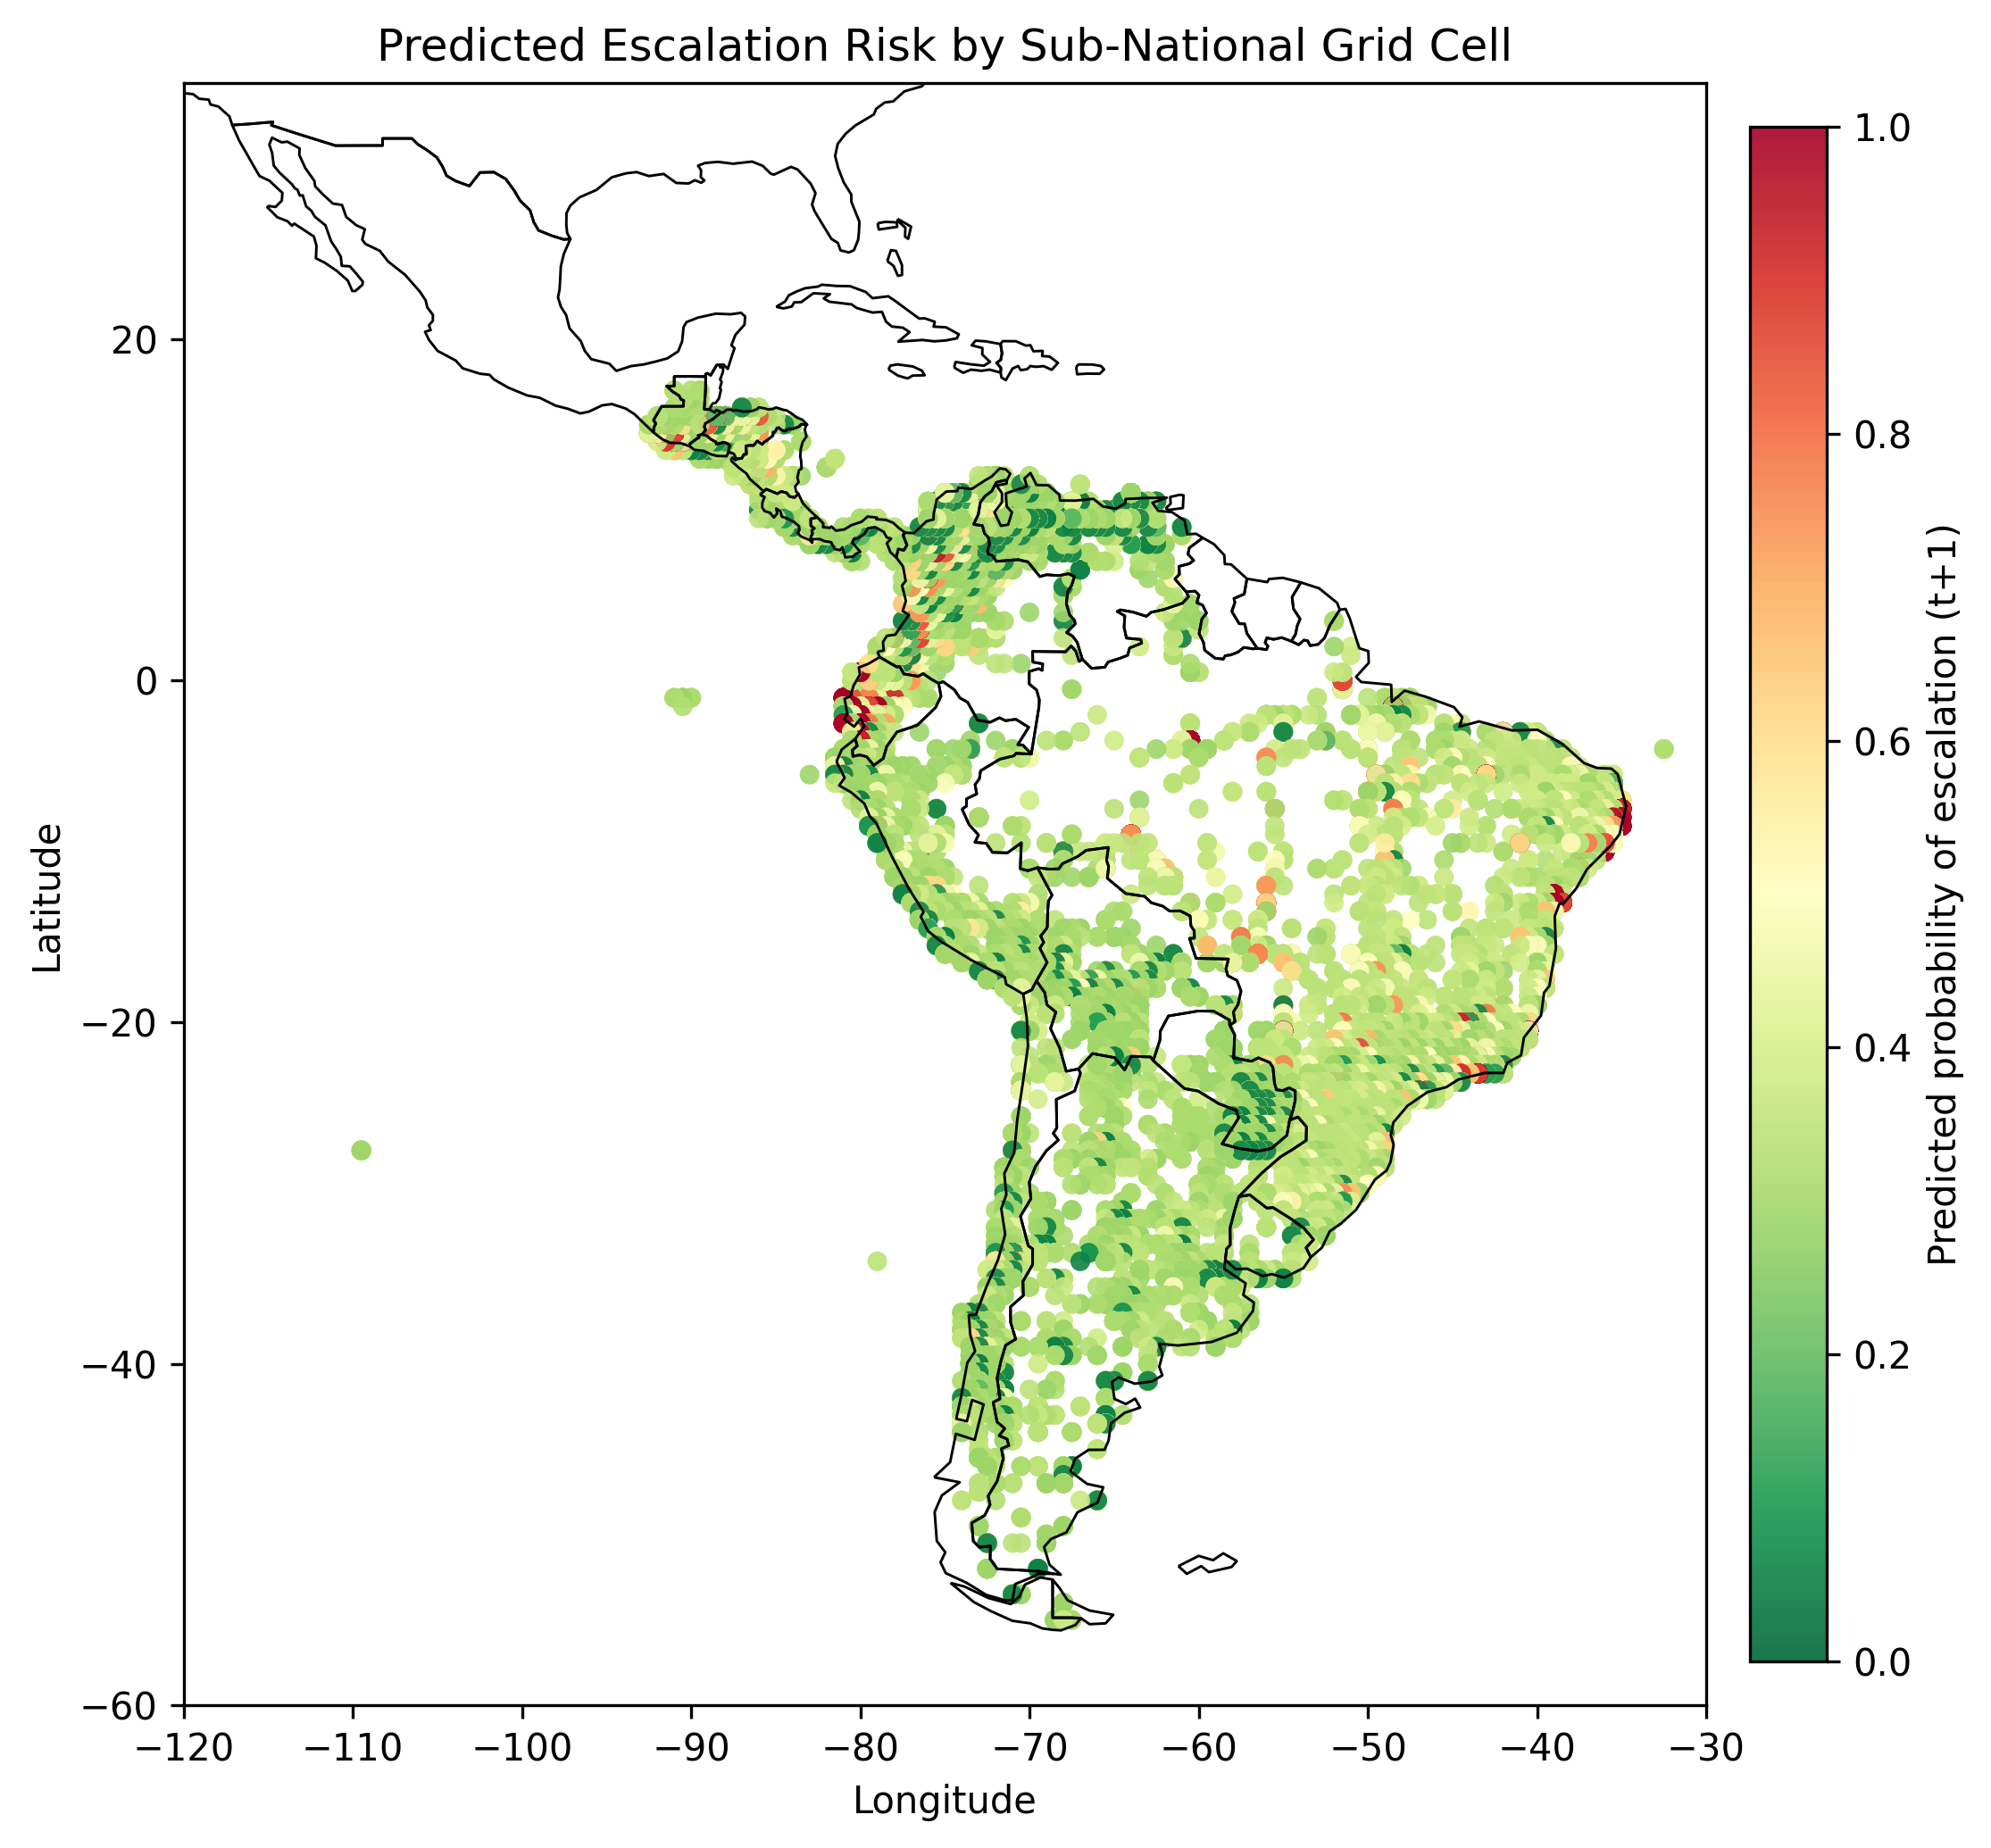
\includegraphics[width=0.70\textwidth]{figures/risk_map_gridcell.png}
\caption{Predicted escalation risk across grid cells, derived from country--month model predictions using ACLED data (2015--2025).}
\label{fig:risk_map}

\vspace{0.25cm}


\includegraphics[width=0.60\textwidth]{figures/pr_curve_logit_test.png}
\caption{Precision--recall curve for escalation prediction on the test dataset (2024--2025).}
\label{fig:prcurve}
\end{figure}

\clearpage

\begin{figure}[H]
\centering

\includegraphics[width=0.70\textwidth]{figures/calibration_plot_test.png}
\caption{Calibration plot comparing predicted escalation probabilities with observed escalation rates across probability bins on the test set (2024--2025).}
\label{fig:calibration}

\vspace{0.25cm}


\includegraphics[width=0.70\textwidth]{figures/xgb_feature_importance_top10.png}
\caption{Top 10 feature importance scores from the XGBoost model.}
\label{fig:xgbimportance}
\end{figure}

\clearpage

\clearpage
\bibliography{refs}
\bibliographystyle{chicago}

\end{document}